Environment reconstruction has been receiving a lot of attention from the research  community, specially using Simultaneous Localization and Mapping (SLAM) procedures. 
%Can be categorized according to the problem methodology in Extended Kalman filters, graph-based optimization and particle filters~\cite{Thrun2008_SLAM}.
A classification can be made by the nature of the sensing devices. While the SLAM problem with depth data may be considered closed, solving it with visual input alone is still an open research question. Furthermore, achieving a solution with spiking neural networks has received little attention despite the efficiency that this approach could provide. Most SLAM solutions only handle static indoor environments, although the vast majority of the world is outdoors and inherently dynamic. Another open question is how to deal with continuously accumulating sensing and/or inference errors, the recovery from which is key for dealing with ever-changing environments. 
%Papers that summarize and explain the mathematical framework of the SLAM problem can be found in the references chapter~\cite{Thrun2008_SLAM,Fuentes-Pacheco2012-slam,durrant2006simultaneous,bailey2006simultaneous}. 

In terms of sensor input, a division of SLAM that uses visual information as the sole external input is, not surprisingly, called \emph{visualSLAM}. In that group of algorithms  there are some that use a single camera, binocular vision, DVS, or RGB-D cameras, to name a few (Figure~\ref{fig:slam:camera-comparison}). 

A conventional camera captures colour information available for a fixed period of time (i.e. a frame). An RGB-D camera captures both colour and depth information; the latter is usually done with laser radars or structured light. A DVS is a visual sensor that emits an event whenever (i.e. dynamically) a pixel senses a change in contrast over time. A benefit of this is that static objects in a scene have a low probability of generating an event.
%The latter is not using only visual information, but it is using just a camera. 

\begin{figure}[h]
  \begin{center}
    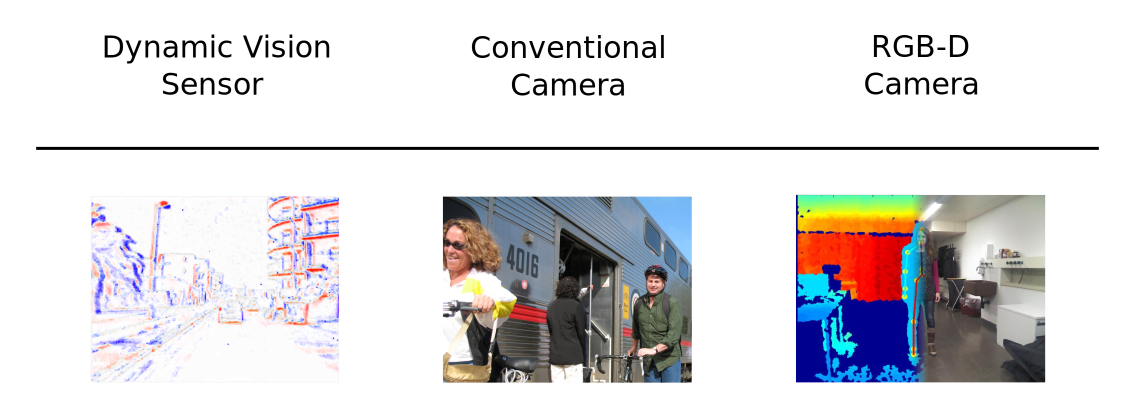
\includegraphics[width=\textwidth]{camera-comparison}
    \caption{Comparison of different visual inputs. Left: a DVS sensor, captures temporal contrast changes in a $\mu s$ scale (red and blue colours). Middle: a conventional camera captures light accumulated during a time window. Right: an RGB-D camera provides depth (left half of the sample image) plus colour (right half) information of a scene.}
    \label{fig:slam:camera-comparison}
  \end{center}
\end{figure}


If only images are used, the correspondence problem arises; where is a feature from one frame located in the next. To solve this, there are mainly two efficient approaches: the first is to use descriptors~\cite{lowe1999object,bay2006surf,alahi2012freak} (i.e. salient features of objects) or to use landmarks~\cite{sola2012impact,frintrop2006attentional} (i.e. full objects). In our approach, the use of visual landmarks is chosen due to neural networks' image recognition capabilities. 


%Spiking neural networks (SNN) need to convert any visual input to spike trains. 
\emph{Event-based 3D SLAM}~\cite{Weikersdorfer2014} is a work that uses a DVS  with RGB-D camera to create a sparse representation of 3D frames. It then uses Bayesian network and condensation particle filter algorithm. They obtain good results with few resources, but they are not using ANNs.

\citeauthor{villaverde2006morphological}~\cite{villaverde2006morphological} report a neural network approach for solving the localization and mapping. An interesting point is the use of Morphological Associative Memories to store and recall morphologically strong-independent patterns. 

Neural networks have also been used to complement other SLAM solutions, for instance by using a NN to better estimate the mapping in presence of noise and errors~\cite{choi2007neural}. A one hidden layer perceptron is used to estimate the uncertainty of the model and increase its accuracy. Another interesting NN extension to SLAM algorithms was reported by \citeauthor{saeedi2011neural}~\cite{saeedi2011neural}, they use a neural network to fuse the results of SLAM algorithms performed by multiple robots. The NN cluster representations into an occupancy grid map.

Hippocampus-based navigation studies has been developed by the neuroscience community. A simulation of a model of place cells is tested in a small robot through neural networks~\cite{burgess1997robotic}, with good results in terms of self-localization and environment recognition. A review of the different aspects of the theory behind hippocampus navigation was published by \citeauthor{sunderhauf2010learning}~\cite{sunderhauf2010learning}. 

A bio-inspired algorithm to solve the SLAM problem is \emph{RatSLAM}, it's based on the hippocampus of rodents, which has been studied for its involvement in navigation tasks. Pose is estimated by activity of place cells arranged in a competitive attractor neural network. If visual information is familiar with respect to a place cell, the latter gets excitatory input. Odometry helps select current active place cells. Results in semi-Cartesian space, on-line incremental, distributed representation via place cells~\cite{rat-slam,milford2008robot}.